\section{Implementation}
\label{sec:implementation}

\begin{figure}
    \centering
    \begin{subfigure}[t]{\columnwidth}
        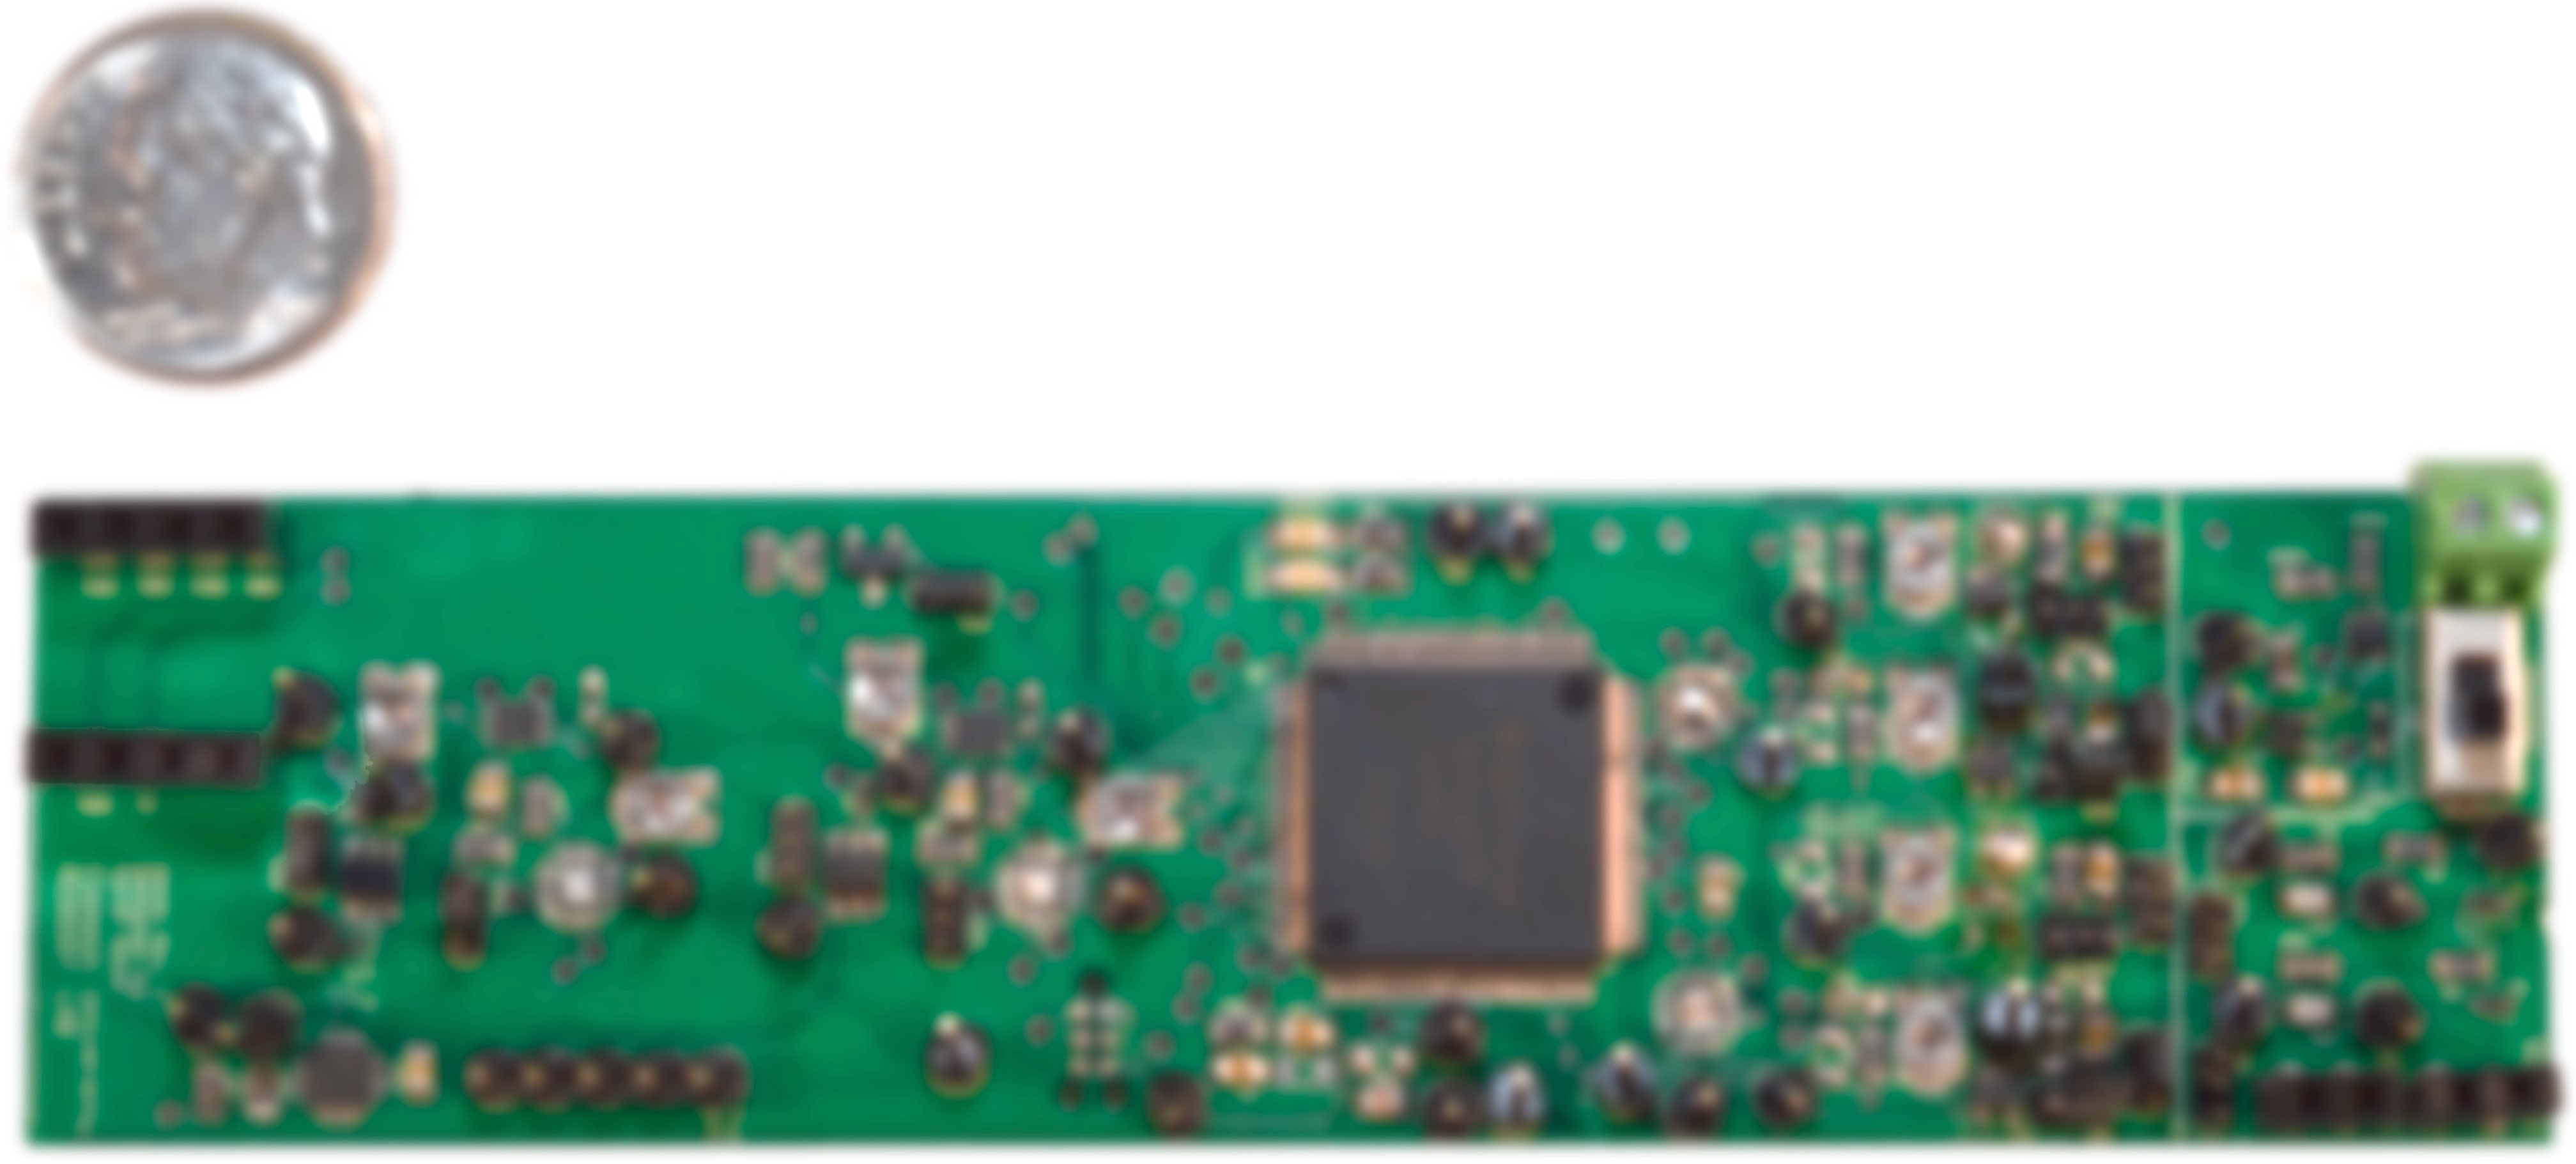
\includegraphics[width=\columnwidth]{figs/board_lossy.jpg}
        \caption{ \sysname prototype PCB.}
        \label{fig:pcb}
    \end{subfigure}

    \begin{subfigure}[t]{\columnwidth}
        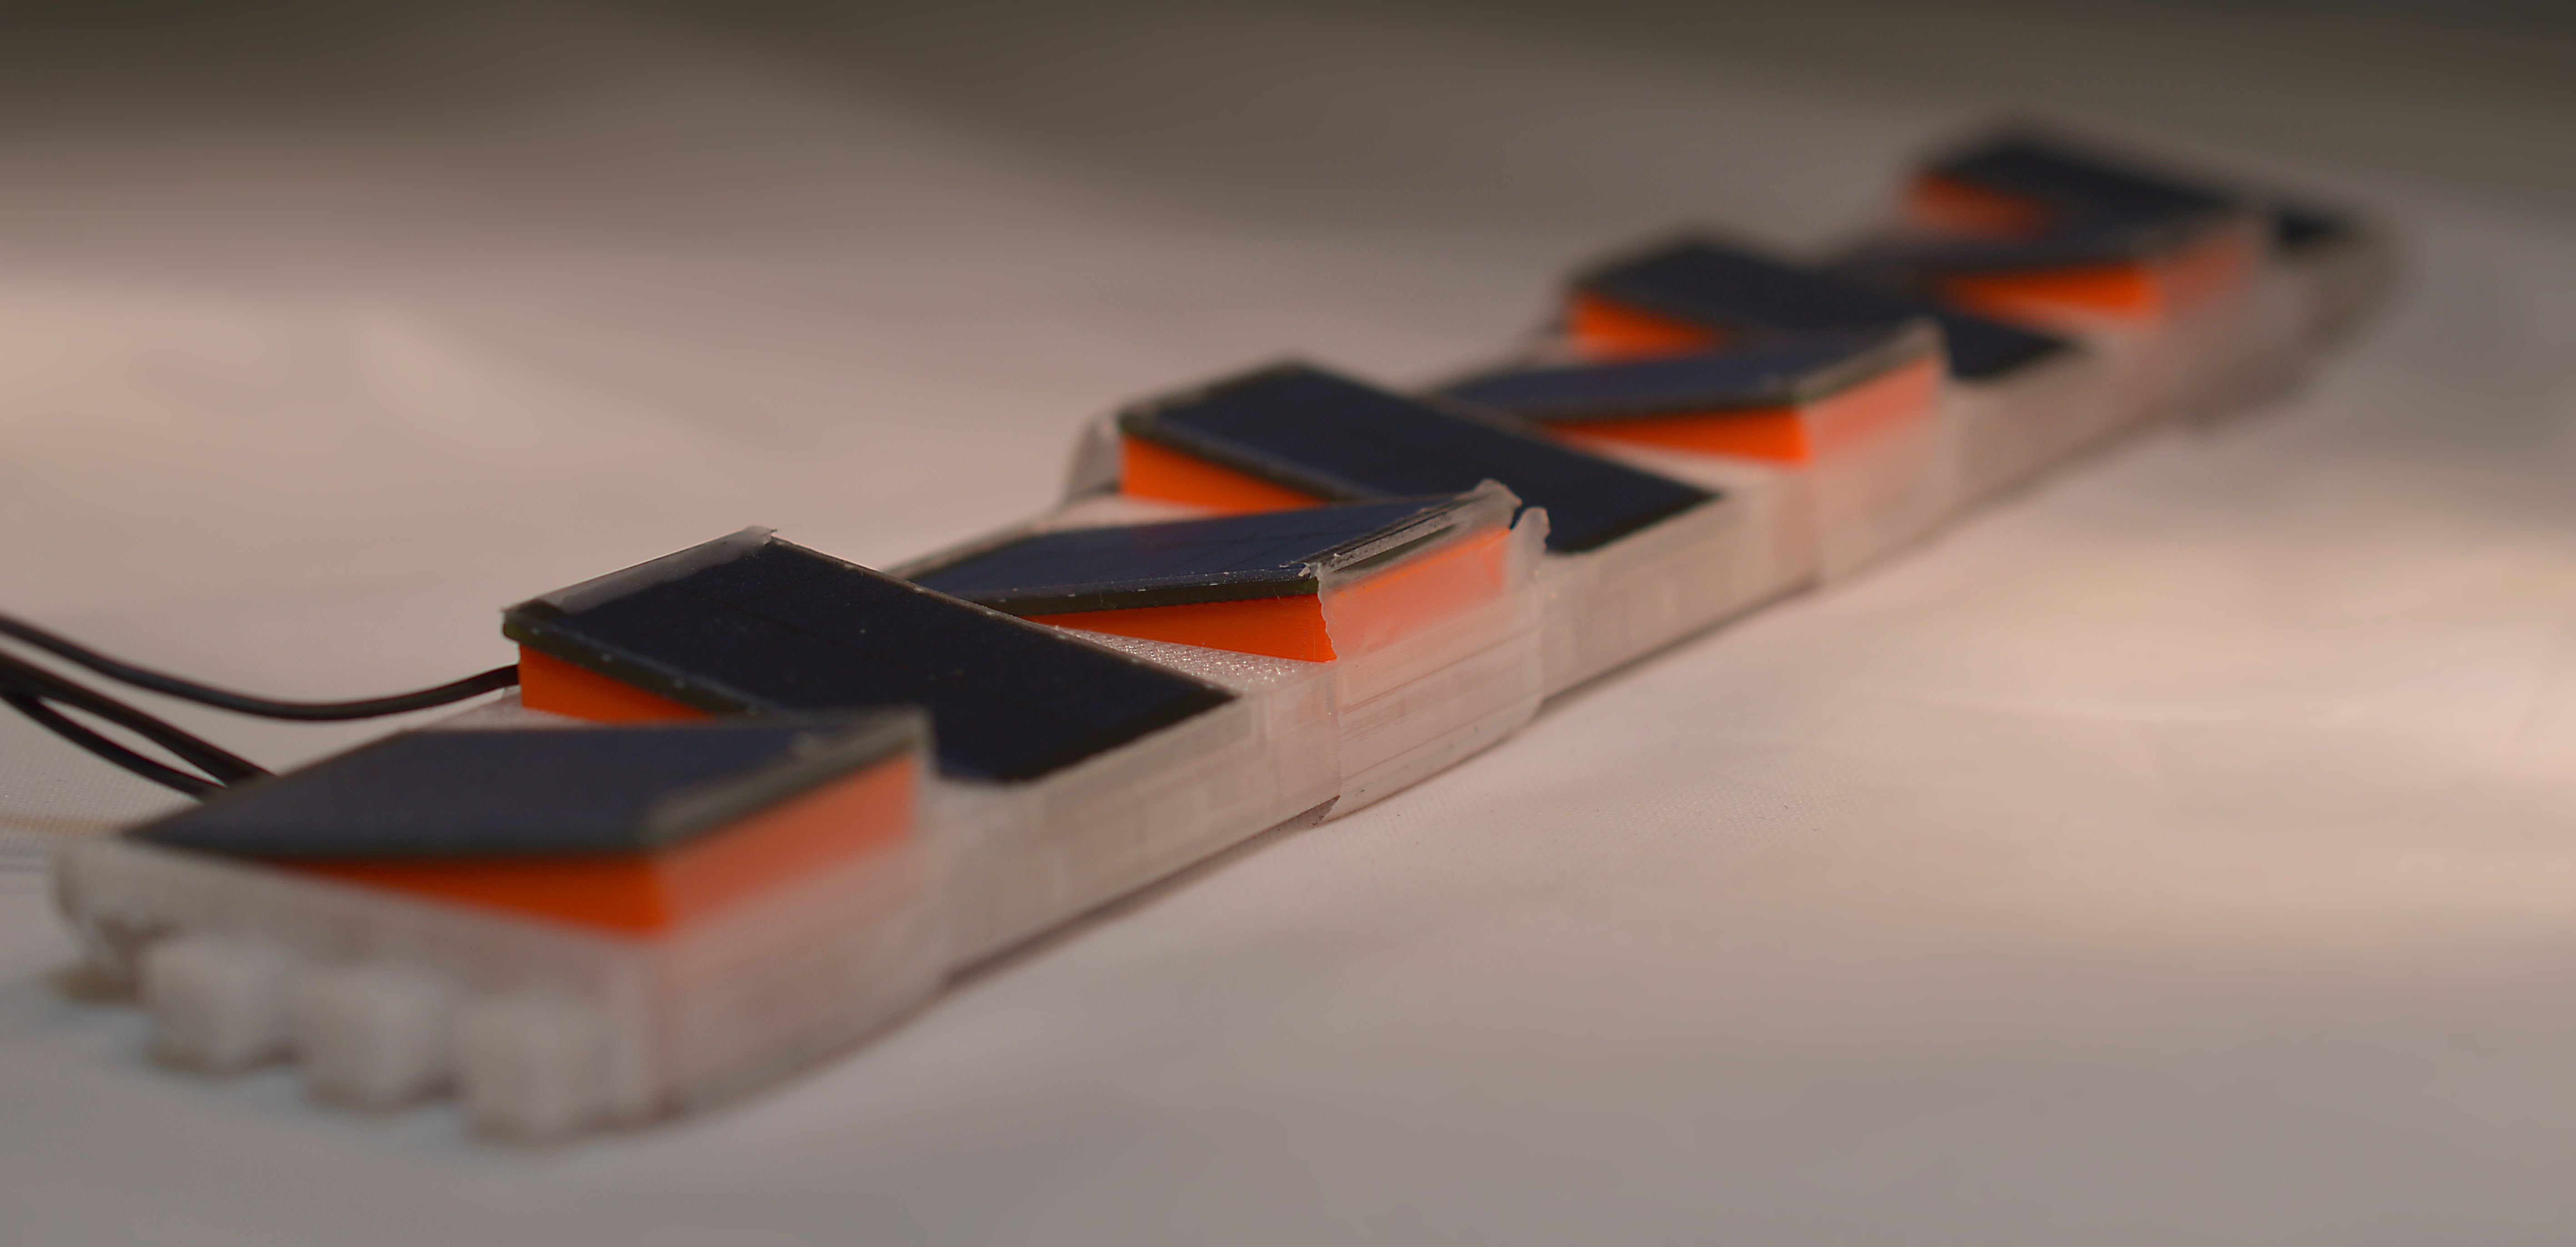
\includegraphics[width=\columnwidth]{figs/panels_lossy.jpg}
        \caption{3D printed solar panel enclosure with angled slots for solar energy harvesters.}
        \label{fig:mounting}
    \end{subfigure}
    \caption{\sysname implementation (some details obscured for anonymization). \label{fig:prototype}}
\end{figure}

We have implemented a prototype \sysname sensor for use in evaluating our approach, including custom hardware in the form of a Printed Circuit Board (PCB) (shown in \figref{fig:pcb}, firmware for managing the doorway sensing application, and a custom 3D printed doorway mounting system that holds the assembled PCB and solar panels in a slim profile \figref{fig:mounting}.

\noindpar{Hardware:} Our prototype hardware integrates eight (8) RL-55x70 solar panels (70.00mm x 55.00mm) from Seeed and a custom printed circuit board~(PCB) held together by a 3D-printed plastic enclosure, detailed later in this section.
The prototype's hardware is composed of an MSP430FR6989 microcontroller from Texas Instrument's (TI) FRAM line of ultra-low-power processors.
The newest FRAM-based MSP430's have several advantages over previous models: lower sleep-mode currents, shorter wake-up latencies, and faster nonvolatile FRAM.
Using the faster wake-up capabilities, \sysname is driven entirely by interrupts and remains asleep most of the time to conserve energy when not in use.
The solar panels are connected in series to increase the harvesting voltage, allowing for greater volatility in voltage which makes it easier to recognize features of the signal. This comes at the cost of increased harvesting current.
The differentiator circuitry is made using nano-power TI TLV3691 comparators and a passive RC filter network. The RC filter network is tunable using trim potentiometers pre-installation, or digital potentiometers in deployment.
The \sysname PCB also has a TI CC1101 radio for communication.
The hardware used in the \sysname prototype, shown in \figref{fig:pcb}, is not prohibitively expensive or obtrusive.
% solar panels are expensive: $14 for 8, device cost is 19.37
The total cost of the current prototype, including all PCB, parts, assembly costs, and solar panels is \$33.37 per unit if ordered in quantities of 1000.

\noindpar{Firmware:}
The \sysname firmware implements the detection algorithm discussed in \secref{sec:system}. Monitoring the interrupts from the detectors, and analyzing the waveform once triggered are the main tasks.
The firmware is designed to be ultra low power even in active mode, and has low computational complexity, offloading the bulk of the detection to the differentiator circuits.
The \sysname firmware is composed of 398 lines of commented C code, compiling to a 2110 byte image. This code size comprises only 1.6\% of the available code space on the MSP430FR6989 (128KB), leaving ample room for implementing custom tasks, recognizers, or multiprogramming operating systems.  

\noindpar{Mechanical Design:}
The 3D printed mounting system (shown in \figref{fig:mounting}) is made of PLA plastics and contains the PCB, solar cells, and necessary wiring connecting them.
\sysname's 3D printed enclosure measures \SI{13.2}{\centi\meter} by \SI{47.0}{\centi\meter} by \SI{1.0}{\centi\meter} at its thickest point. The enclosure provides a nesting place for the solar cells, pointing downward.
The angle of the solar cell slots is set such that some solar cells tend toward the entry, while the rest toward the exit.

All software, firmware, hardware schematics and layouts, and 3D printed mounting system will be made freely available at publication time.
